%%%%%%%%%%%%%%%%%%%%%%%%%%%%%%%%%%%%%%%%%%%%%%%%%%%%%%%%%%%%%%%%%%%%%%%%%%%%%%%%%%%
% Team:
% Union
% Members: 
% Bernie Huan, Jim Lan, Hoang Tan, Kenny Hsu, Rahul Aditya, Tan Phat, Wei
% Relative files:
% Main.tex, Background_Union.tex, Library.bib, Union_Background_Chart_1.png, Union_Background_Chart_2.png, Union_Background_Chart_3.png, Union_Background_Chart_semi.png, Union_Background_Chart_sup1.png, Union_Background_Chart_sup2.png, Union_Background_Chart_sup3.png, Union_Background_Chart_WSD.png
% Note:
% Do not compile this file compile Main.tex to get the pdf file instead.
%%%%%%%%%%%%%%%%%%%%%%%%%%%%%%%%%%%%%%%%%%%%%%%%%%%%%%%%%%%%%%%%%%%%%%%%%%%%%%%%%%%

\subsection{Automatic creation of metadata}

\textit{\footnotesize Author:Bernie Huan, Jim Lan, Hoang Tan, Kenny Hsu, Rahul Aditya, Tan Phat, Wei.}\\

We are producing a program that automatically generate and extract metadata with natural language processing. 
We also strive to generate XML files with metadata extracted. 
In the best scenario, we will even try to create a search engine together with other groups. 
Also, creating a sutiable interface and structure with some finctions for users is necessary. 
Following discussion is our literature review on natural language processing.

\begin{figure*}[ht]
	\begin{center}
		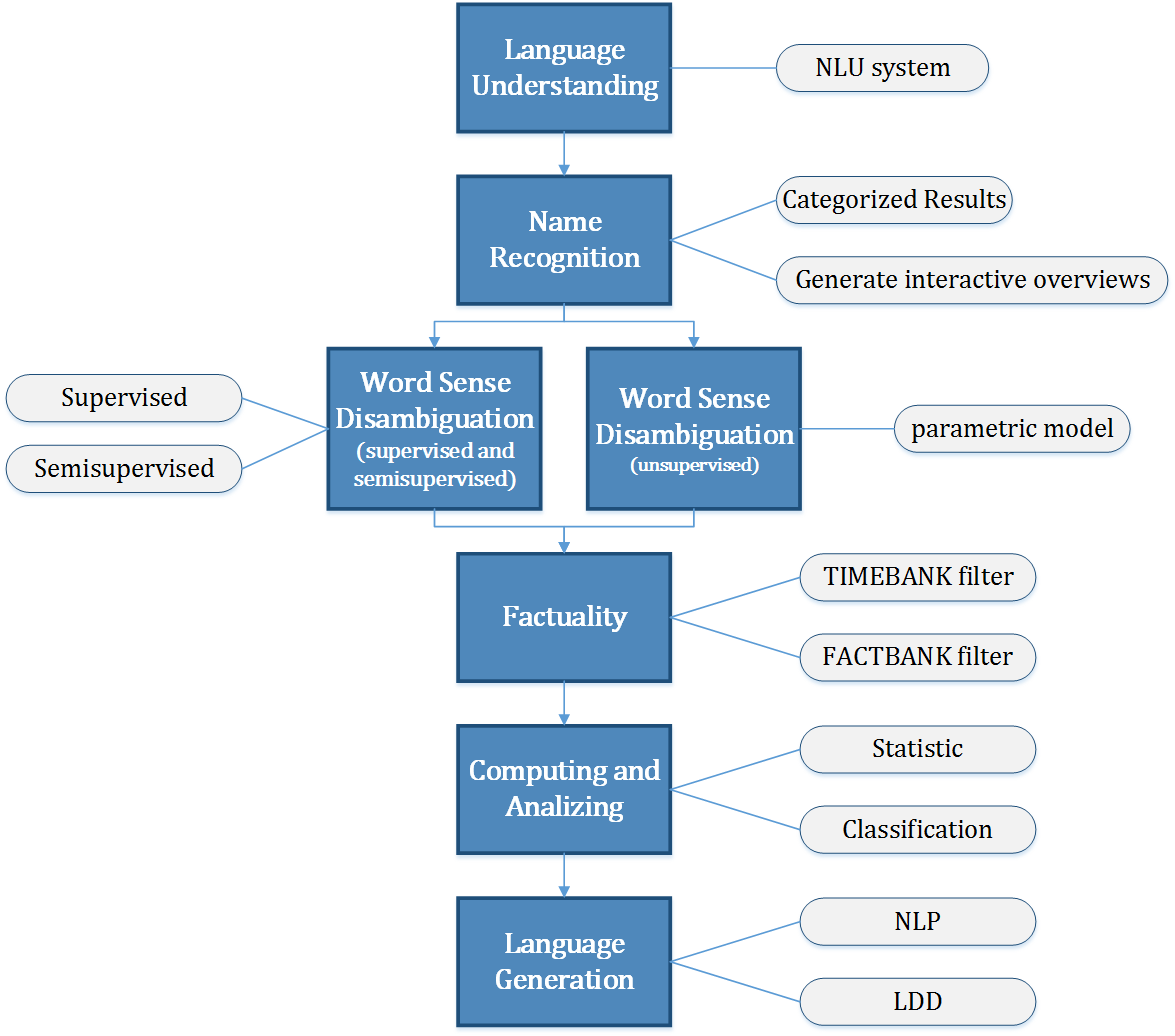
\includegraphics[width=1.8\columnwidth]{Union_Background_Chart_1}
	\end{center}
	\caption{The process of metadata creation.}
\end{figure*}

\subsubsection*{Language understanding}

Natural language understanding (NLU) is a subtopic of natural language processing in artificial intelligence that deals with machine reading comprehension, it's considered an AI-hard problem.

For a machine to understand language, it first has to develop a mental map of words, their meanings and interactions with other words. It needs to build a dictionary of words, and understand where they stand semantically and contextually, compared to other words in their dictionary. To achieve this, each word is mapped to a set of numbers in a high-dimensional space, which are called “word embeddings”. Similar words are close to each other in this number space, and dissimilar words are far apart. Some word embeddings encode mathematical properties such as addition and subtraction.

After the machine has learned word embeddings, the next problem to tackle is the ability to string words together appropriately in small, grammatically correct sentences which make sense. This is called language modeling. Language modeling is one part of quantifying how well the machine understands language.

For example, given a sentence “I am eating pasta for lunch.”, and a word “cars”, if the machine can tell you with high confidence whether or not the word is relevant to the sentence “cars” is related to this sentence with a probability 0.01 and I am pretty confident about it, then that indicates that the machine understands something about words and contexts.

An even simpler metric is to predict the next word in the sentence. Given a sentence, for each word in its dictionary the machine assigns a probability of the word’s likeliness to appear next in the sentence. For example: “I am eating (     ).” To fill in the blank, a good language model would likely give higher probabilities to all edibles like “pasta”, “apple”, or “chocolate”, and it would give lower probability to other words in the dictionary which are contextually irrelevant like “taxi”, “building”, or “music”.

When users search for a sentence, how does the program understand the certain inputs of text? We could build a natural language understanding (NLU) system, in which the system's rules for semantic interpretation are learnt automatically from training data, which uses a set of possible yes-no questions that can be applied to data items.
After that, it follows rules for selecting the best questions at any node on the basis of training data by using a method for pruning trees to prevent over-training.

\subsubsection*{Name Recognition}

If users search for the word "Turkey", the results could be a country or an animal. 
The meaning is totally different and definitely make users very confused if he or she is not very familiar with the word "Turkey". 

There are a lot of misunderstandings like this if users search some words which have multiply meanings. 
Sometimes, the results are fully unrelated and this situation is always annoying. 
That would be troublesome when we count frequency of certain words to rank them.

Therefore, it is significantly crucial for a program to totally understand what users want by name recognition in natural language processing, finally they can find out the results much quicker and will not be confused anymore.

The method to improve the problem above is "categorize the words based on different subjects, topic, or genres" by using online database and python program. 
Metadata is limited in digital libraries and web resources, try to enlarge them with meaningful, organized and desired categories \cite{Kules2006}.

Besides dealing with mutiple-meaning words, the most important part of name recognition is to recognize the special names and terms such as locations, people name, country, even company names and academic terms.
Therefore, it is better for search engine to know what user want and huge name corpus are necessary. 
Plus, this work also can assist previous work.

With above effort, users' exploration and overviews of information could be better supported. It will be very convenient to find the results we want and lower the possibility of misunderstandings if users are not very familiar with finding the appropriate result in specific fields.
\cite{TunThuraThet2010} Users don't need to filter the results which are ranked by browsing frequency popularity but can just obtain the information and relevance by clicking the specific categories and some reasonable choices.

Plus, creating some choices for users is also vital because this make the searching much more oragnized. 
For example, if there are a lot of subtitles such as abstract, introduction, method, or references in some standard research articles, try to make some choices so that the users can easily find out what they want. 
There are a lot of different standard articles in the world.
 Making a suitable choices if someone want to creat a personalzed search engine and interface. 

Also, users are able to choose multiply fields if the results include a lot of relevant fields. 
That's a big motivation for people to handle these problems. 

A lot of online services have done similar tasks before. 
Thus, creating and using an online databases or automated metadata creation are to be recommended. 
The reason is there are many advantages, including integrating with the other cloud services or scaling with what users need such as how to categorize the categories. 
It is beneficial for people who would like to create a convenient and personalized database or metadata.\\\\\\


\todo[inline]{A summary on list format can be motivated, but then each item need to be brief and you should not introduce anything new like UMLS in it.}

\subsubsection*{Factuality}

In the process of producing metadata, which should be the most precise information and representing the text, validity of such metadata must be checked. Therefore, tools for fact checks are developed based on linguistic techniques. 

The tool could detect facts and excludes authors' subjective opinions \cite{Agerri2014}. From the authors's perspective, the two main set of tools having such functions is TIMEBANK and FACTBANK. (yes, the authors used capitalized name)

TIMEBANK was first proposed in \cite{pustejovsky2003timebank}. 
The idea was based on that English language has different tenses which could be exploited as signals for fact check. 
An example below could help to clarify the ideas. Let's examine these sentences:

\begin{itemize}
	\item I will go to Chimei museum tomorrow.
	\item Chimei museum is near Tainan District.
	\item I was in UK in 2012.
\end{itemize}

The first sentence is simple future tense which implies something has never actually happened, the second sentence is simple present tense which can directly imply facts, and the last sentence is in simple past tense which is about something already happened (which is facts), but is no longer a fact right now, so such fact must be used with caution. 

The reason for introducing such tool is that even scientific research articles can be glittering with subjective comments, opinions or even assumption from authors \cite{schultze2000confessional}. In addition to TIMEBANK, many other tools can be another filter for fact extraction. \cite{Dave2003mining} Identify words, clauses and phrases that show emotional state of the authors. 

The choice in expression of facts could also be a helpful indicator to show whether authors are subjectively supporting a cause, an opinion and so on \cite{Wiebe2005}. Among these mentioned approaches, this paper highly favors creation a kind of thesaurus compiled of linguistic signaling for non-factually statements such as FACTBANK, which is built by \cite{Sauri2009}. 
Following example shows how subjective statements can be picked out.

\begin{itemize}
	\item Channelization would guarantee high flow velocity in rivers, flooding and consequent degradation of riparian community (1a).
	\item Funding agencies would be happy with big entrepreneurs, instead of small and medium enterprises (1b).
	\item Tolerance to dictatorship would has negative influences on anarchist movement (2a).
	\item Tolerance to dictatorship would doom anarchist movement (2b).
\end{itemize}

It is easy to find in statement (1a) is an absolute fact. 
Statement (1b) is however affected by emotional state of authors. 
After re-writing (1b) into: Funding agencies lend more money with lower interest rate to big entrepreneurs, instead of small 
and medium enterprises,sentence (1b) become a face-based statement. 
In another case, statement (2a) is a fact-based statement while in statement (2b), authors are stressing their dislike toward dictatorship.

Fact checks in language generation is a new field but many useful tools have been developed. Each of them has their own function and could complement each others. In the limit of this study, we are using both of TIMEBANK and FACTBANK together for fact check.


\subsection{API and search engine}
An API is short-hand of  application programming interface, which include components to define a process of communication and data processing on computer. 
It is necessary to create a search engine as we mentioned at the beginning of this report.
A good example of API is HAPI on Python. 
According to \cite{Kochanov201615}, HAPI is a library included in Python. 
As the library has a collection of defined process, it allow users and other parties (which could be robots or others users at other ends) to interact with each other.
Main functions of the HAPI have been including sending uploads, data filtration and other manipulation. 
The outcomes of such process can be formatted with variable forms. 
As described by \cite{Hedbrant20162206}, programming interface can include following systems:
\begin{itemize}
	\item SOAP: Simple Object Access Protocol
	\item REST: Representational State Transfer
	\item UDDI: Universal Description, Discovery, and Integration
	\item WSDL: Web Service Definition Language
\end{itemize}
	Other programing system can be included as well. 
	SOAP is among a field attracting many recent researches. 
	A good review about SOAP could be found from the work of \cite{Hsieh2009424}. 
	SOAP has important roles in field monitoring as handling a huge amount of data can be trouble some in many senses. 
	SOAP in conjunction with other programming techniques, such as distributed computing, are employed because it can solve 3 problems listed below:
	\begin{itemize}
		\item Is the system scalable: 
		There are systems that suitable for a fixed amount of data, but not functional when the need of expending data storage comes in place. 
		With such system, programmers will have to build another system. 
		That would be a waste of human resource, time and money.
		\item Is the system reliable: 
		In other words, can data be stored safely. 
		Many data obtained in field monitoring are expensive. 
		Therefore, it is important to make sure data will be always there whenever a need of retrieval arisen. 
		Also, the data may be retrieved, processed and formatted by many people involved in the system.
		A reliable system will not be broken down easily and foremost, data will be safely stored.
		\item Is the system accessible: 
		This matter can be put in two questions 1- When we need to use the data, is it hard to retrieve it from the system. 
		Do we need trained personal to do that job.
		And if we do, which level of training is necessary. 
		2- How many people can access the system. 
		
	\end{itemize}
	It is proven in many engineering projects, the application of SOAP can help overcome these problems, especially in term of increasing accessiblity.
	\subsubsection{Search engine}
	As mentioned above, creating a search engine is an example of API application. 
	In this section we feel the need to give an example of how to create search engine with API. 
	We found an inspirational example from the work of \cite{Noei2016135}. 
	Although the authors not just using SOAP, but also more advanced Object Access Protocol such as Java, it shows that OAP in general improve code and design. 
	Consequently, it saves time and effort in developing new program.
	The authors also offer EXAF (EXample Applications Finder) so that program developers can find other examples that fits their interest.
	
\newpage % Ends the current page and causes all figures and tables to be printed